%%%%%%%% ICML 2023 EXAMPLE LATEX SUBMISSION FILE %%%%%%%%%%%%%%%%%

\documentclass{article}

% Recommended, but optional, packages for figures and better typesetting:
\usepackage{microtype}
\usepackage{graphicx}
\usepackage{subfigure}
\usepackage{booktabs} % for professional tables
\usepackage{comment}

\usepackage{tikz}
% Corporate Design of the University of Tübingen
% Primary Colors
\definecolor{TUred}{RGB}{165,30,55}
\definecolor{TUgold}{RGB}{180,160,105}
\definecolor{TUdark}{RGB}{50,65,75}
\definecolor{TUgray}{RGB}{175,179,183}

% Secondary Colors
\definecolor{TUdarkblue}{RGB}{65,90,140}
\definecolor{TUblue}{RGB}{0,105,170}
\definecolor{TUlightblue}{RGB}{80,170,200}
\definecolor{TUlightgreen}{RGB}{130,185,160}
\definecolor{TUgreen}{RGB}{125,165,75}
\definecolor{TUdarkgreen}{RGB}{50,110,30}
\definecolor{TUocre}{RGB}{200,80,60}
\definecolor{TUmagenta}{RGB}{175,110,150}
\definecolor{TUmauve}{RGB}{180,160,150}
\definecolor{TUbeige}{RGB}{215,180,105}
\definecolor{TUorange}{RGB}{210,150,0}
\definecolor{TUbrown}{RGB}{145,105,70}

% hyperref makes hyperlinks in the resulting PDF.
% If your build breaks (sometimes temporarily if a hyperlink spans a page)
% please comment out the following usepackage line and replace
% \usepackage{icml2023} with \usepackage[nohyperref]{icml2023} above.
\usepackage{hyperref}


% Attempt to make hyperref and algorithmic work together better:
\newcommand{\theHalgorithm}{\arabic{algorithm}}

\usepackage[accepted]{icml2023}

% For theorems and such
\usepackage{amsmath}
\usepackage{amssymb}
\usepackage{mathtools}
\usepackage{amsthm}

\setlength{\abovedisplayskip}{0pt}
\setlength{\belowdisplayskip}{0pt}
\setlength{\abovedisplayshortskip}{0pt}
\setlength{\belowdisplayshortskip}{0pt}


% if you use cleveref..
\usepackage[capitalize,noabbrev]{cleveref}

%%%%%%%%%%%%%%%%%%%%%%%%%%%%%%%%
% THEOREMS
%%%%%%%%%%%%%%%%%%%%%%%%%%%%%%%%
\theoremstyle{plain}
\newtheorem{theorem}{Theorem}[section]
\newtheorem{proposition}[theorem]{Proposition}
\newtheorem{lemma}[theorem]{Lemma}
\newtheorem{corollary}[theorem]{Corollary}
\theoremstyle{definition}
\newtheorem{definition}[theorem]{Definition}
\newtheorem{assumption}[theorem]{Assumption}
\theoremstyle{remark}
\newtheorem{remark}[theorem]{Remark}

\newcommand{\R}{\mathbb{R}}

% Todonotes is useful during development; simply uncomment the next line
%    and comment out the line below the next line to turn off comments
%\usepackage[disable,textsize=tiny]{todonotes}
\usepackage[textsize=tiny]{todonotes}


% The \icmltitle you define below is probably too long as a header.
% Therefore, a short form for the running title is supplied here:
\icmltitlerunning{Project Report Template for Data Literacy 2023/24}

\renewcommand{\vec}[1]{\begin{bmatrix}#1\end{bmatrix}}

\begin{document}

\twocolumn[
\icmltitle{An Analysis of Wind Energy Potential in the North Sea}

% It is OKAY to include author information, even for blind
% submissions: the style file will automatically remove it for you
% unless you've provided the [accepted] option to the icml2023
% package.

% List of affiliations: The first argument should be a (short)
% identifier you will use later to specify author affiliations
% Academic affiliations should list Department, University, City, Region, Country
% Industry affiliations should list Company, City, Region, Country

% You can specify symbols, otherwise they are numbered in order.
% Ideally, you should not use this facility. Affiliations will be numbered
% in order of appearance and this is the preferred way.
\icmlsetsymbol{equal}{*}

\begin{icmlauthorlist}
\icmlauthor{Mohammad Fadel Berakdar}{equal,first}
\icmlauthor{Gwendolyn Neitzel}{equal,second}
\icmlauthor{David Voigt}{equal,third}
\icmlauthor{Alireza Yahyanejad}{equal,fourth}
\end{icmlauthorlist}

% fill in your matrikelnummer, email address, degree, for each group member
\icmlaffiliation{first}{Matrikelnummer 6117917, mohammad-fadel.berakdar@student.uni-tuebingen.de, MSc Bioinformatics}
\icmlaffiliation{second}{Matrikelnummer 5425507, gwendolyn.neitzel@student.uni-tuebingen.de, MSc Mathematik}
\icmlaffiliation{third}{Matrikelnummer 5416770, david.voigt@student.uni-tuebingen.de, MSc Computer Science}
\icmlaffiliation{fourth}{Matrikelnummer 6645496, alireza.yahyanejad@student.uni-tuebingen.de, MSc Computer Science}

% You may provide any keywords that you
% find helpful for describing your paper; these are used to populate
% the "keywords" metadata in the PDF but will not be shown in the document
\icmlkeywords{Machine Learning, ICML}

\vskip 0.3in
]

% this must go after the closing bracket ] following \twocolumn[ ...

% This command actually creates the footnote in the first column
% listing the affiliations and the copyright notice.
% The command takes one argument, which is text to display at the start of the footnote.
% The \icmlEqualContribution command is standard text for equal contribution.
% Remove it (just {}) if you do not need this facility.

%\printAffiliationsAndNotice{}  % leave blank if no need to mention equal contribution
\printAffiliationsAndNotice{\icmlEqualContribution} % otherwise use the standard text.

\begin{abstract}
%\textcolor{magenta}{
%Put your abstract here. Abstracts typically start with a sentence motivating why the subject is interesting. Then mention the data, methodology or methods you are working with, and describe results.}
In the face of climate change, it is widely agreed that energy production has to rely on more
sustainable and renewable forms of harnessing energy. Offshore wind turbine parks play a crucial
role in increasing the share of green energy. This paper explores probabilistic methods of assessing
the wind energy potential and potential trends of data collected on Helgoland by considering wind
speeds as a Weibull distributed random variable. Further, for forecasting, the monthly expected wind
power density is extrapolated using a Gaussian process regression model.
\end{abstract}

\section{Introduction}\label{sec:intro}
With the rising need for clean and sustainable energy due to climate change, offshore wind energy is
playing an important role in the future energy mix of many European countries \citep{eu_comm}.  In
the context of Germany, the North Sea is considered a prime location for offshore wind parks, with
41 farms already established and many more in planning \citep{wind-farms}.  For assessing the
viability of offshore wind parks, an often used metric is the wind power density \cite{wang2021wind,
miao2020117382, mohammadi2016assessing}.  In this paper, we follow \citet{mohammadi2016assessing} by
considering the wind speed as a Weibull distributed random variable (Section \ref{sec:weibull}).
Further, we conduct a trend analysis (Section \ref{sec:weibull}) on the change of the parameters of
the yearly wind speed distributions and look for evidence for the phenomenon of global terrestrial
stilling, that is, a decrease in the global mean annual surface wind speed starting in the 1980s
\cite{stilling}.  As proposed by \citet{mohammadi2016assessing}, we compute the wind power density
probabilistically as the expectation of the monthly and yearly Weibull distributions (Section
\ref{sec:power-density}). We then employ a Gaussian process regression model for the prediction of
future wind power densities (Section \ref{sec:gp}). In Section \ref{sec:results}, we present the
results of applying the aforementioned methods to real-world data.\footnote{The complete source of
this paper can be found in our \href{https://github.com/FadelBerakdar/DataLiteracyProject}{repositoriy}.}

\section{Data}\label{sec:data}
%\textcolor{magenta}{In this section, describe \emph{what you did}. Roughly speaking, explain what data you worked with, how or from where it was collected, it's structure and size.Explain your analysis, and any specific choices you made in it. Depending on the nature of your project, you may focus more or less on certain aspects. If you collected data yourself, explain the collection process in detail. If you downloaded data from the net, show an exploratory analysis that builds intuition for the data, and shows that you know the data well. If you are doing a custom analysis, explain how it works and why it is the right choice. If you are using a standard tool, it may still help to briefly outline it. Cite relevant works.}You can use the \verb|\citep| and \verb|\citet| commands for this purpose \citep{mackay2003information}.

The wind speed data used in this paper was collected by the \href{https://www.dwd.de}{DWD} on
\href{https://www.openstreetmap.org/?mlat=54.1750&mlon=7.8920#map=15/54.1750/7.8920}{Helgoland},
spanning the years from 1996 to 2022. The wind speed is recorded at a temporal resolution of
ten-minutes\footnote{Averaged over the last ten-minute interval.}, with the anemometer being $4.38
\mathrm{m}$ above ground. Averaged over the whole measurement period, the data has a yearly mean
completeness of about $91\%$. Notably, the year 2019 is missing $88\%$ of its measurements. We
consider this, and a noticeable drop in the yearly wind speed mean and variance of the following
years, as evidence that the measurement process was changed, and therefore discard them. Notably,
the years 1996 to 1998 have a completeness of about $3\%, 85\%$ and $84\%$, respectively. For
preventing a distorting effect on the Weibull distribution estimations, we also did not consider
these years for our analysis, thereby improving the yearly mean completeness to $99\%$. For handling
outliers, we dropped measurements exhibiting a z-score $> 8$.

\section{Methods}\label{sec:methods}

\subsection{Fitting of the Weibull Distribution and Trend Analysis}\label{sec:weibull}
Based on the observed wind data, we model the wind speed probability distribution both on a monthly
and yearly basis.  Whilst there are several other models, like the three-parameter Weibull
distribution or the normal distribution for fitting wind speed frequencies, the most prominent one
is the two-parameter Weibull distribution \cite{review, statanalysis, mohammadi2016assessing}.  For
the scale parameter $\lambda >0$ and shape parameter $\beta >0$, the probability density function
(PDF) and cumulative density function (CDF) are given by
\begin{align}
    \label{eq:pdf}
    p(v) &=
    \begin{cases}
        \frac{\beta}{\lambda} \left( \frac{v}{\beta}\right)^{\beta-1} 
        \exp{ \left( -\left(\frac{v}{\lambda}\right)^\beta \right)} & \text{  for } v>0 \\
        0 & \text{ else}
    \end{cases} \\
    \label{eq:cdf}
    P(v)&=
    \begin{cases}
        1- \exp{\left(-\left(\frac{v}{\lambda}\right)^\beta \right)} & \text{  for } v>0 \\
        0 & \text{ else}
    \end{cases}.
\end{align}
Via the gamma function, $\Gamma(z)= \int_{0}^{\infty}t^{z-1} \mathrm{e}^{-t}dt$, 
the $k$-th raw moment and the variance of a random variable $V$ with Weibull distribution can be expressed as follows: 
\begin{align}  
    \mathrm{E}[V^k] &= \lambda^k \Gamma \left( 1 + \frac{k}{\beta} \right) \label{eq:n-raw-moment} \\
    \mathrm{Var}[V] &= \lambda^2 \left[  \Gamma \left( 1 + \frac{2}{\beta}\right) \label{eq:var}
    - \Gamma^2 \left( 1 + \frac{1}{\beta}\right)\right].
\end{align}

We determine the parameters $\lambda$ and $\beta$ for every month and year using the maximum
likelihood method applied to \eqref{eq:pdf} \cite{mohammadi2016assessing}.  Due to the seasonal
variability of wind speed, the long-term trend analysis is conducted on the yearly (rather than
monthly) estimated wind speed PDFs. For this, we employ a least-squares linear regression and assess
the statistical significance through a two-sided permutation test at the $5\%$ level.  Since the two
Weibull parameters fully characterize the distribution, we are then able to use this analysis to
infer trends in other quantities of interest, like mean and standard deviation.

\subsection{Wind Power Density}\label{sec:power-density}

The wind power density is often used as an approximation of the physical upper limit of how much
energy a wind turbine is able to harness \cite{wang2021wind, mohammadi2016assessing,
miao2020117382}. The power density is given by
\begin{align}\label{eq:power}
    \mathrm{P} &= \frac{1}{2} \cdot \rho \cdot \mathrm{v}^3 \\
    [\mathrm{P}] &= [\rho] \cdot [\mathrm{v}^3] = \frac{\mathrm{kg}}{\mathrm{m}^3} \cdot \frac{\mathrm{m}^3}{\mathrm{s}^3} = \frac{\mathrm{W}}{\mathrm{m}^2}
\end{align}
where $\rho$ is the air density, and $\mathrm{v}$ is the wind speed. Notice that the wind power
density is independent of the area covered by the wind turbine's rotors. Using equation
\eqref{eq:power} the expected power density can be found by calculating the expected value under the
given distribution $p(\mathrm{v})$ as follows:
\begin{align}\label{eq:power-expectation}
    E[P] &= \int_{\mathrm{v}_\mathrm{min}}^{\mathrm{v}_\mathrm{max}} \frac{1}{2} \cdot \rho \cdot \mathrm{v}^3 \cdot p(\mathrm{v}) \, \mathrm{dv} \\
    &= \frac{1}{2} \cdot \rho \cdot \int_{\mathrm{v}_\mathrm{min}}^{\mathrm{v}_\mathrm{max}} \mathrm{v}^3 \cdot p(\mathrm{v}) \, \mathrm{dv}.
\end{align}
For a range of $v_\mathrm{min} = 0 \, \frac{\mathrm{m}}{\mathrm{s}}$ and $v_\mathrm{max} = \infty \,
\frac{\mathrm{m}}{\mathrm{s}}$, the solution to this integral is given by the third raw-moment as
shown in \eqref{eq:n-raw-moment}. However, in using these limits, we would assume that wind turbines
are able to convert energy during arbitrarily high or low wind speeds. Thus, a more sensible
assumption is to use the so-called cut-in $\mathrm{v}_\mathrm{in}$ and cut-out wind speed
$\mathrm{v}_\mathrm{out}$ of wind turbines. For a generic wind turbine, a common assumption is
$\mathrm{v}_\mathrm{in} \in [2, 4] \, \frac{\mathrm{m}}{\mathrm{s}}$ and $\mathrm{v}_\mathrm{out}
\in [20, 23] \, \frac{\mathrm{m}}{\mathrm{s}}$ \cite{dupont2017, wang2021wind}.

\subsection{Gaussian Process Regression}\label{sec:gp}
For forecasting, we employ a Gaussian process regression (GPR) model to perform a time-series
regression on the monthly estimated power density and extrapolate future values. Thereby, we assume
that the wind speed data $Y \in \mathbb{R}^N$ is from a latent function $f: \mathbb{R}^N \rightarrow
\mathbb{R}^N$ with some added measurement noise: $y = f(x) + \epsilon$. The GPR framework consists
of a Gaussian process as prior, multivariate Gaussian likelihood and Gaussian process posterior
conditioned on the data
\cite{rasmussen-williams-gp}:
\begin{align}
    \label{eq:gp_prior}
    p(f) &= \mathcal{GP}(f; 0, k), \\
    \label{eq:gp_likelihood}
    p(y \mid f) &= \mathcal{N}(Y; f, \sigma^2 I), \\
    \label{eq:gp_posterior}
    p(f \mid Y) &= \mathcal{GP}(f; m', k') \propto p(Y \mid f) \cdot p(f).
\end{align}
The resulting posterior (and prior) distribution collapses into a multivariate normal distribution
when evaluated at some new locations $X' \in \mathbb{R}^M$.

\section{Results}\label{sec:results}
%\textcolor{magenta}{In this section, outline your results. At this point, you are just stating the outcome of your analysis. You can highlight important aspects (``we observe a significantly higher value of $x$ over $y$''), but leave interpretation and opinion to the next section. This section absolutely \emph{has} to include at least two figures.}\\

\subsection{Weibull Parameter Estimation and Trend Analysis}
\label{sec:trend}

For the available years (1999-2018) we estimated the parameters of the Weibull distribution on a monthly and yearly basis. 
\begin{figure}
    \centering 
    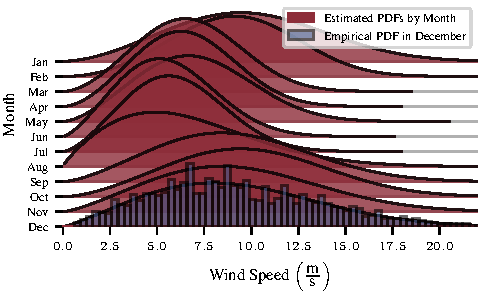
\includegraphics{fig/monthly_weibull.pdf}
    \caption{The monthly estimated Weibull distributions in the year 2010. The parameter $\lambda$ decreases in summer, whilst $\beta$ decreases, resulting in a shift to the left and lower standard deviation.}
    \label{fig:monthly_weibull}
\end{figure}
Figure \ref{fig:monthly_weibull} depicts the resulting PDFs for the months of 2010 as well as the
empirical histogram in December.  When applying the square root rule to the number of bins,
this fit has an expected relative error per bin of $18 \%$.  Averaged over the monthly and yearly
distributions, the expected relative error per bin is  $23 \%$ and $22 \%$, respectively.

\begin{figure}
    \centering
    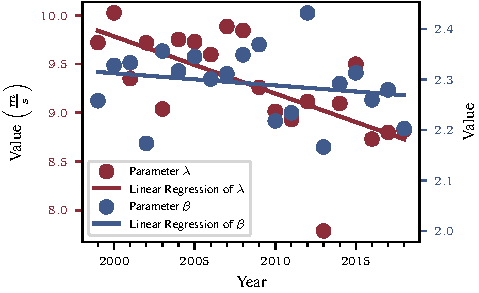
\includegraphics{fig/linreg_parameters.pdf}
    \caption{The linear regression of the yearly Weibull parameters shows a noticeable decrease in 
 \textcolor{TUred}{$\lambda$}, but less so in \textcolor{TUdarkblue}{$\beta$}.}
    \label{fig:lin_reg}
\end{figure}

The least-squares linear regression of the yearly parameters can be seen in Figure
\ref{fig:lin_reg}.  It shows a decrease of the parameter $\lambda$ of $-0.059\frac{m}{s}
\frac{1}{\mathrm{yr}}$ with an RMSE of $0.42\frac{m}{s}$.  For $\beta$, the slope is $-0.002
\frac{1}{\mathrm{yr}}$, with an RMSE of $0.07  \frac{m}{s}$.  At the $5\%$ level of the two-sided
permutation test, the null hypothesis that there is no linear trend in the development of the
parameter $\lambda$ can be rejected (p-value$=0.001$), so the observation is statistically
significant.  For the parameter $\beta$, however, the p-value is $0.383$, so we cannot reject the
null hypothesis.  Assuming the trend observed in $\lambda$ and the empiric mean $\bar \beta=2.29$
for $\beta$, we derive the following trends in other quantities: As the mean  and standard deviation
are proportional to $ \lambda$, we can infer a linear trend of $-0.052 \frac{m}{s}
\frac{1}{\mathrm{yr}}$ and  $-0.024 \frac{m}{s} \frac{1}{\mathrm{yr}}$, respectively.
%Further, the probabilities of wind speed below $ 3 \frac{m}{s}$ and above $22 \frac{m}{s}$ are especially relevant (Section \ref{sec:power-density}):
%Over the entire $22$ year period, the estimated probabilities change (in a non-linear fashion) from $6.46 \%$ to $8.15 \%$ and from $0.17 \%$ to $0.03 \%$, respectively. 
Further, under these assumptions, the mean power density of the mean wind speed decreases
(non-linearly) from 1999 to 2018 by $30\%$.

\subsection{Expected Power Density}

By using \eqref{eq:power-expectation}, we numerically computed the expected power density under each
of the estimated monthly Weibull distributions with $v_\mathrm{min} = 3 \,
\frac{\mathrm{m}}{\mathrm{s}}$ and $v_\mathrm{max} = 22 \, \frac{\mathrm{m}}{\mathrm{s}}$. The
resulting values can be found as the ground truth in Figure \ref{fig:gp-samples} and
\ref{fig:gp-pred}.

\begin{figure}
    \centering
    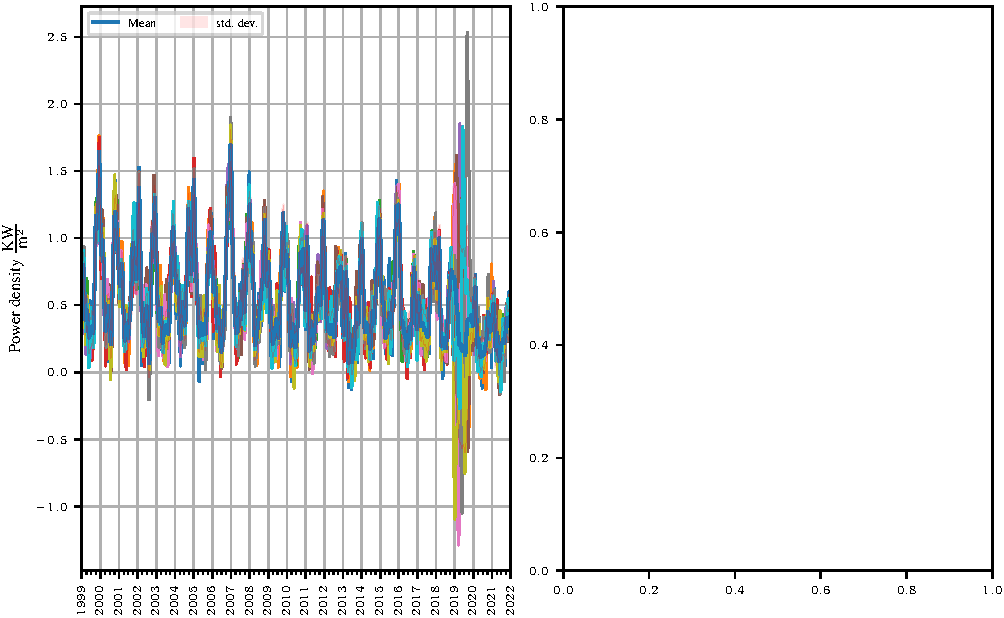
\includegraphics{fig/gp_samples.pdf}
    \caption{The \textcolor{TUdarkblue}{ground truth} data plotted together with three samples $f_i \sim \mathcal{GP}(f; 0, k)$ drawn from the Gaussian Process prior distribution with the added \textcolor{TUred}{mean} $\overline{Y}$ of the data $Y$.}
    \label{fig:gp-samples}
\end{figure}


\subsection{Gaussian Process Regression}
\begin{figure*}[htb!]
    \centering
    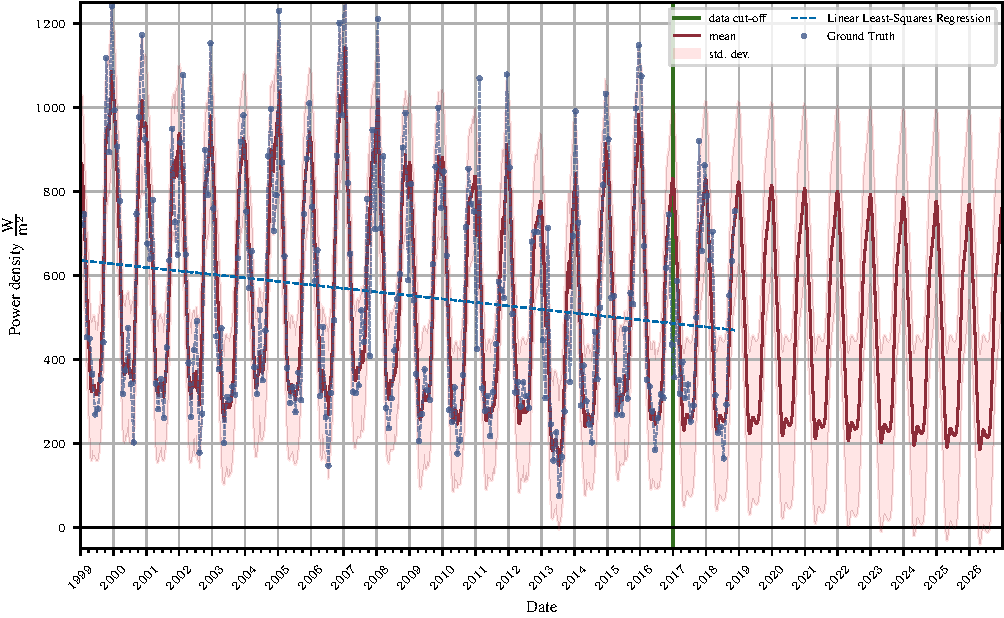
\includegraphics[width=0.975\textwidth]{fig/gp_pred.pdf}
    \caption{The \textcolor{TUred}{mean} and \textcolor{TUred}{standard deviation} of the posterior distribution $\mathcal{N}(f(x); m', k')$ evaluated at $x$ is plotted together with the linearly interpolated \textcolor{TUdarkblue}{ground truth}. Starting at the \textcolor{TUdarkgreen}{data cut-off}, the model is extrapolating (predicting) the power density into the future.}
    \label{fig:gp-pred}
\end{figure*}


%For assessing the viability of wind turbine (parks), one might also be interested in the weekly or daily values  and, even more importantly, in a forecast. Hence, for interpolating the daily expected power density, we employ a Gaussian Process Regression model to perform a time-series regression. In addition to interpolating, we also use the same model for extrapolation and thereby making predictions about the future daily expected power density.
The first step for conducting a GP regression is to decide on a kernel $k$ for the prior
\eqref{eq:gp_prior}. By analysing the plotted raw monthly expected power density, we identify a
yearly periodic trend and a slight global downward trend. The former can be captured by the
Exponential-Sine-Squared kernel (ES) \cite{MacKay1998IntroductionTG}. Supported by the empirical
data, we choose a periodicity of $365 \, \text{days}$ and an amplitude of $350 \,
\frac{\textrm{W}}{\text{m}^2}$. For the length scale, we settle for a rather small value ($< 2 \, $
days) in order to capture local patterns in the periodicity more accurately. For allowing the
amplitude to slowly decay over long periods of time, we multiply the ES kernel by a very smooth
(length scale $> 50 \, \text{years}$) Squared-Exponential (SE) kernel. For reproducing the global
downwards trend observed in section \ref{sec:trend}, we also choose a very smooth
Squared-Exponential kernel with an output scale of $100 \, \frac{\textrm{W}}{\text{m}^2}$. For
accounting for the monthly midterm trend, we add a Rational-Quadratic kernel
\cite{rasmussen-williams-gp} with a scale of $10 \, \frac{\textrm{W}}{\text{m}^2}$ and a length
scale of one month. Finally, the additive kernel, consisting of a White-Noise (WN) and a Matern
kernel (MA) \cite{abramowitz1968handbook}, is responsible for explaining measurement noise in the
data and thus also prevents overfitting. Thereby, the kernel has the form 
$$k = \underbrace{\text{ES} \cdot \text{SE}}_{\text{yearly trend}} 
+ \underbrace{\text{RQ}}_\text{monthly trend} 
+ \underbrace{\text{ES}}_\text{longterm trend} 
+ \underbrace{\text{WN} 
+ \text{MA}}_{\text{noise}}.$$
By drawing samples\footnote{with the mean of the data added.} $f_i \sim
\mathcal{GP}(f; 0, k)$ from the prior distribution \eqref{eq:gp_prior}, we gauge how accurately our
kernel choice fits to the given data. The results are shown in Figure \ref{fig:gp-samples}. We can
observe that the amplitude and periodicity of some of the samples mirrors the data's in an accurate
manner, supporting our choice of hyperparameters. After conditioning the Gaussian process prior on
the normalised data, we obtain the posterior distribution $\mathcal{GP}(f; m', k')$
\eqref{eq:gp_posterior}. The evaluated posterior mean and standard deviation can be found in Figure
\ref{fig:gp-pred}. We can observe that the mean function is following the periodicity of the ground
truth without overfitting extreme power densities. Furthermore, the uncertainty of the model
(standard deviation) increases gradually the further the prediction is from the data. Notably, the
model also captures the global downward trend. When comparing the prediction to the test data in the
years 2017 and 2018, we can observe that the prediction fits the ground truth accurately and all
data points are well within one standard deviation of the mean.

\section{Discussion \& Conclusion}\label{sec:conclusion}
%\textcolor{magenta}{Use this section to briefly summarize the entire text. Highlight limitations and problems, but also make clear statements where they are possible and supported by the analysis.}
In this paper, we analysed the wind energy potential of the island Helgoland in the North Sea.  We
have found a decrease in the mean annual wind speed of $-0.052 \frac{m}{s}  \frac{1}{\mathrm{yr}}$,
consistent with the global phenomenon of terrestrial stilling \cite{stilling}. In this location, a
reversal in the stilling, as  was observed globally \cite{stilling-reversal}, could not be found. If
the trend prevails, diminishing wind energy production is to be expected at this particular
location.  Further, we have shone light on the monthly variations in expected power density, a
valuable insight for evaluating potential contribution to the overall energy supply.  Lastly, we
explored Gaussian process regression as a tool for extrapolating the expected power density.  We
have found that it is adequate for this purpose, being able to adapt to a variety of subtrends and
cyclical behaviours due to the explicit and flexible choice of the prior kernel function. By
comparing the test data with the prediction, we consider the fit to be accurate and the uncertainty
quantification realistic.

However, there are some shortcomings. One of the inherent limitations of the GPR is that it yields
functions mapping onto $\R$, while the power density is only limited to $\R_+$.
%Further, we conducted an interpolation of daily values based on monthly data, which does not take the inter-day variability into account. For the purpose of extrapolating daily power densities, 
%it might be advisable in further work to rely on daily data to begin with, complicating the choice of the kernel.  
Another important limitation is that our data was recorded at a height of $4.38 \mathrm{m}$, whereas
the real height of wind turbines can exceed $100 \mathrm{m}$. One commonly applied rule of thumb to
mitigate this issue is multiplying the wind speeds by the factor $\left(\frac{h}{4.38 \mathrm{m}}
\right)^{0.14}$ or the power density by its cube, where $h$ is the  proposed hub height of a turbine
\citep{statanalysis}. However, this is far from exact, as the winds at different heights could be
subject to different circulations.  Furthermore, we did not take the direction of the wind into
account and made the simplification that wind turbines are always perfectly aligned.  Also, for
equation \eqref{eq:power}, we assumed a constant air pressure rather than considering the monthly
changing pressure.  Lastly, with the use of the maximum-likelihood method, we assumed the
independence of measurements. While this is generally not given, we were still able to produce
adequate estimations.

\section*{Contribution Statement}
David Voigt conducted the Gaussian process regression. 
Gwendolyn Neitzel was mainly concerned with the Weibull model fitting and the trend analysis.
Mohammad Fadel Berakdar focused on the data preprocessing. Alireza Yahyanejad worked on data loading.
All authors were involved in data exploration and jointly wrote the report. 
%\textcolor{magenta}{Explain here, in one sentence per person, what each group member contributed. For example, you could write: Max Mustermann collected and prepared data. Gabi Musterfrau and John Doe performed the data analysis. Jane Doe produced visualizations. All authors will jointly write the text of the report. Note that you, as a group, are collectively responsible for the report. Your contributions should be roughly equal in amount and difficulty.}

%\section*{Notes} 
%\textcolor{magenta}{
%Your entire report has a \textbf{hard page limit of 4 pages} excluding references. (I.e. any pages beyond page 4 must only contain references). Appendices are \emph{not} possible. But you can put additional material, like interactive visualizations or videos, on a GitHub repo (use \href{https://github.com/pnkraemer/tueplots}{links} in your PDF to refer to them). Each report has to contain \textbf{at least three plots or visualizations}, and \textbf{cite at least two references}. More details about how to prepare the report, including how to produce plots, cite correctly, and how to ideally structure your GitHub repo, will be discussed in the lecture, where a rubric for the evaluation will also be provided.
%}

\pagebreak

\bibliography{bibliography}
\bibliographystyle{icml2023}

\end{document}


% This document was modified from the file originally made available by
% Pat Langley and Andrea Danyluk for ICML-2K. This version was created
% by Iain Murray in 2018, and modified by Alexandre Bouchard in
% 2019 and 2021 and by Csaba Szepesvari, Gang Niu and Sivan Sabato in 2022.
% Modified again in 2023 by Sivan Sabato and Jonathan Scarlett.
% Previous contributors include Dan Roy, Lise Getoor and Tobias
% Scheffer, which was slightly modified from the 2010 version by
% Thorsten Joachims & Johannes Fuernkranz, slightly modified from the
% 2009 version by Kiri Wagstaff and Sam Roweis's 2008 version, which is
% slightly modified from Prasad Tadepalli's 2007 version which is a
% lightly changed version of the previous year's version by Andrew
% Moore, which was in turn edited from those of Kristian Kersting and
% Codrina Lauth. Alex Smola contributed to the algorithmic style files.
